%!TEX root = ../../master.tex
\section*{Workshops}

Workshops have been a created to give the students direct hands-on learning experiences. This approach is selected since both Docker and Kubernetes uses a command-line tool, that has to be learned through use. Furthermore, the Resilience and Load testing workshop adds command-line tools that has to be used in order to run these kinds of tests. \\

\renewcommand*{\arraystretch}{2}
\noindent\begin{tabular}{p{6cm}p{7.5cm}}

\fbox{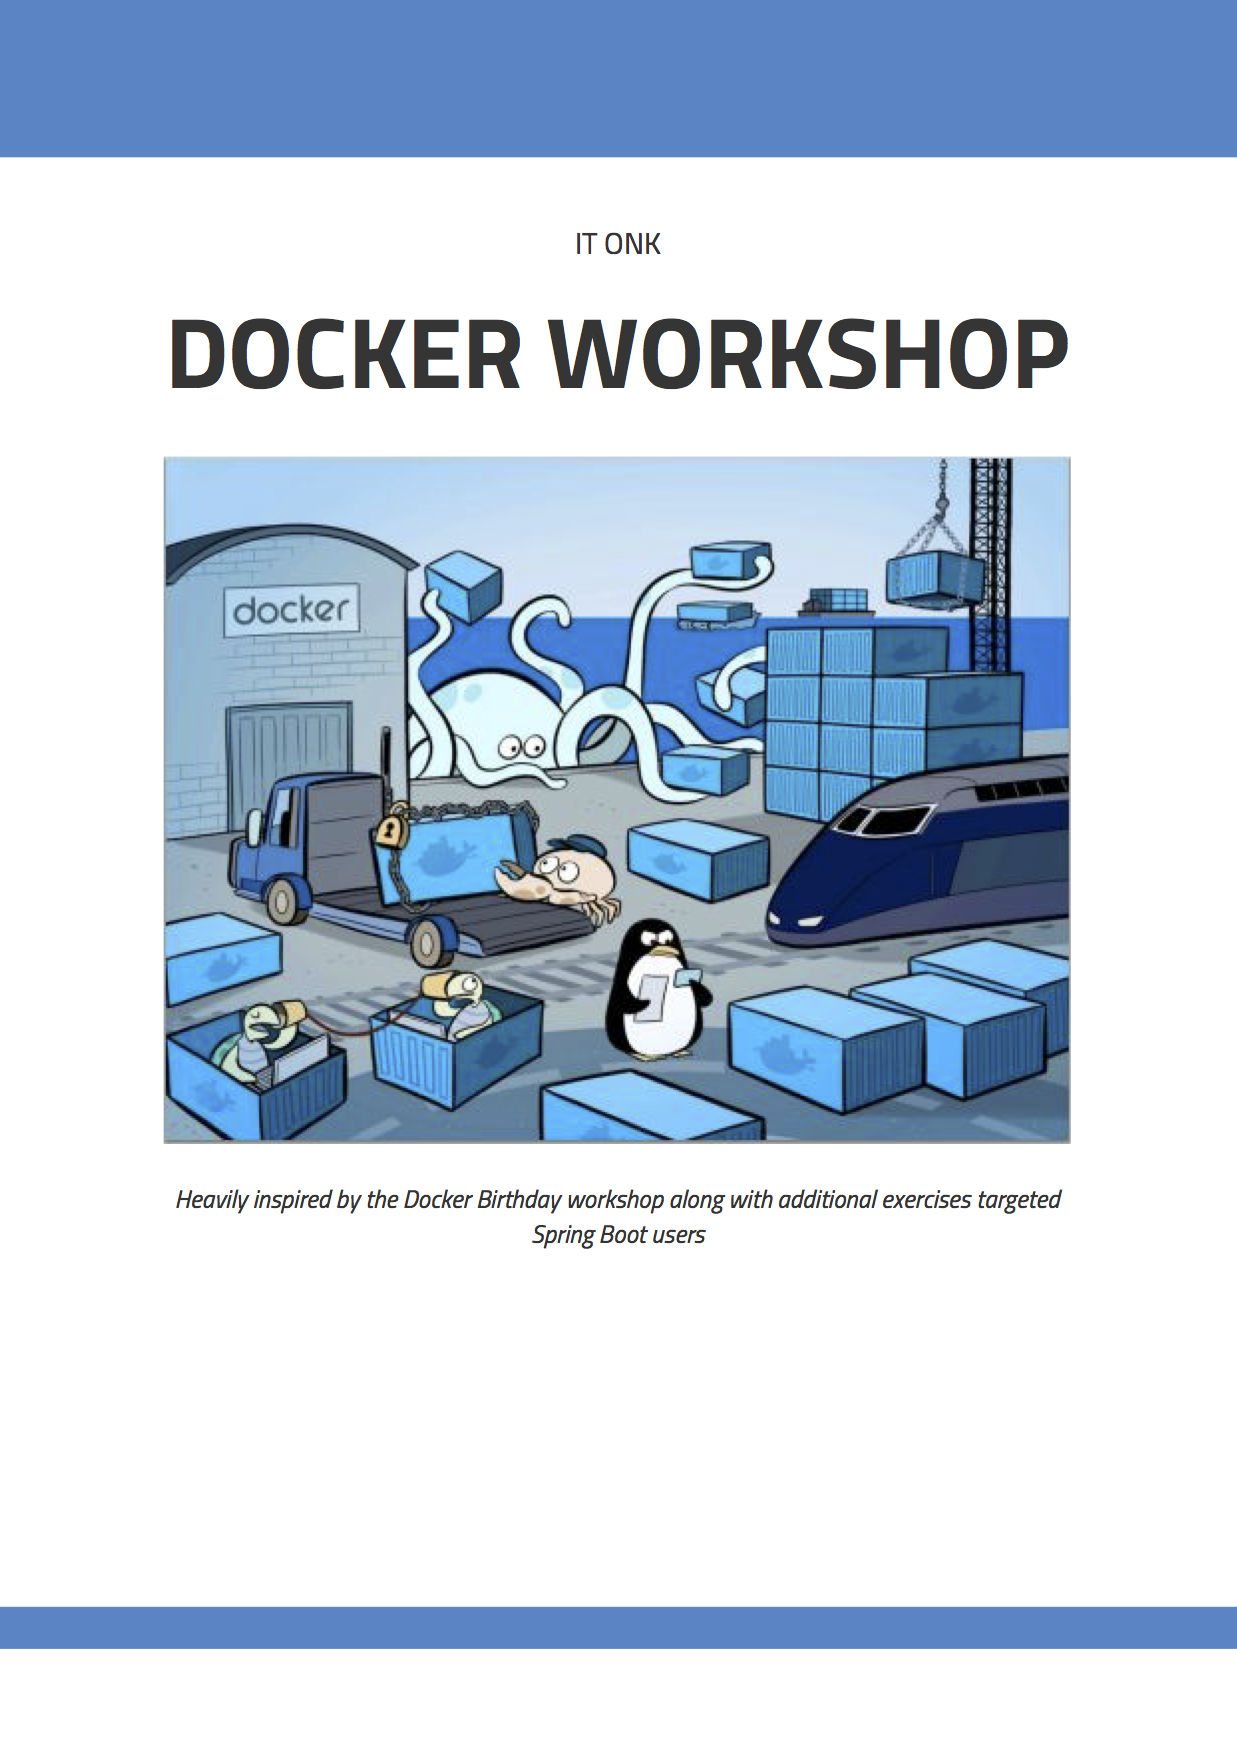
\includegraphics[align=t,width=5.5cm]{figures/workshop/module2_docker_workshop}} & \textbf{Docker workshop} \newline \textit{(17 sider)} \newline This workshop will give the student the ability to create docker images, run these images as containers, and lastly build and package a Java Spring Boot application into a container and running it on a Raspberry Pi. Furthermore this workshop will provide more detailed insights in how Docker works, along with developing the students confidence in using Docker thereby improving their skills.  \\ 




\fbox{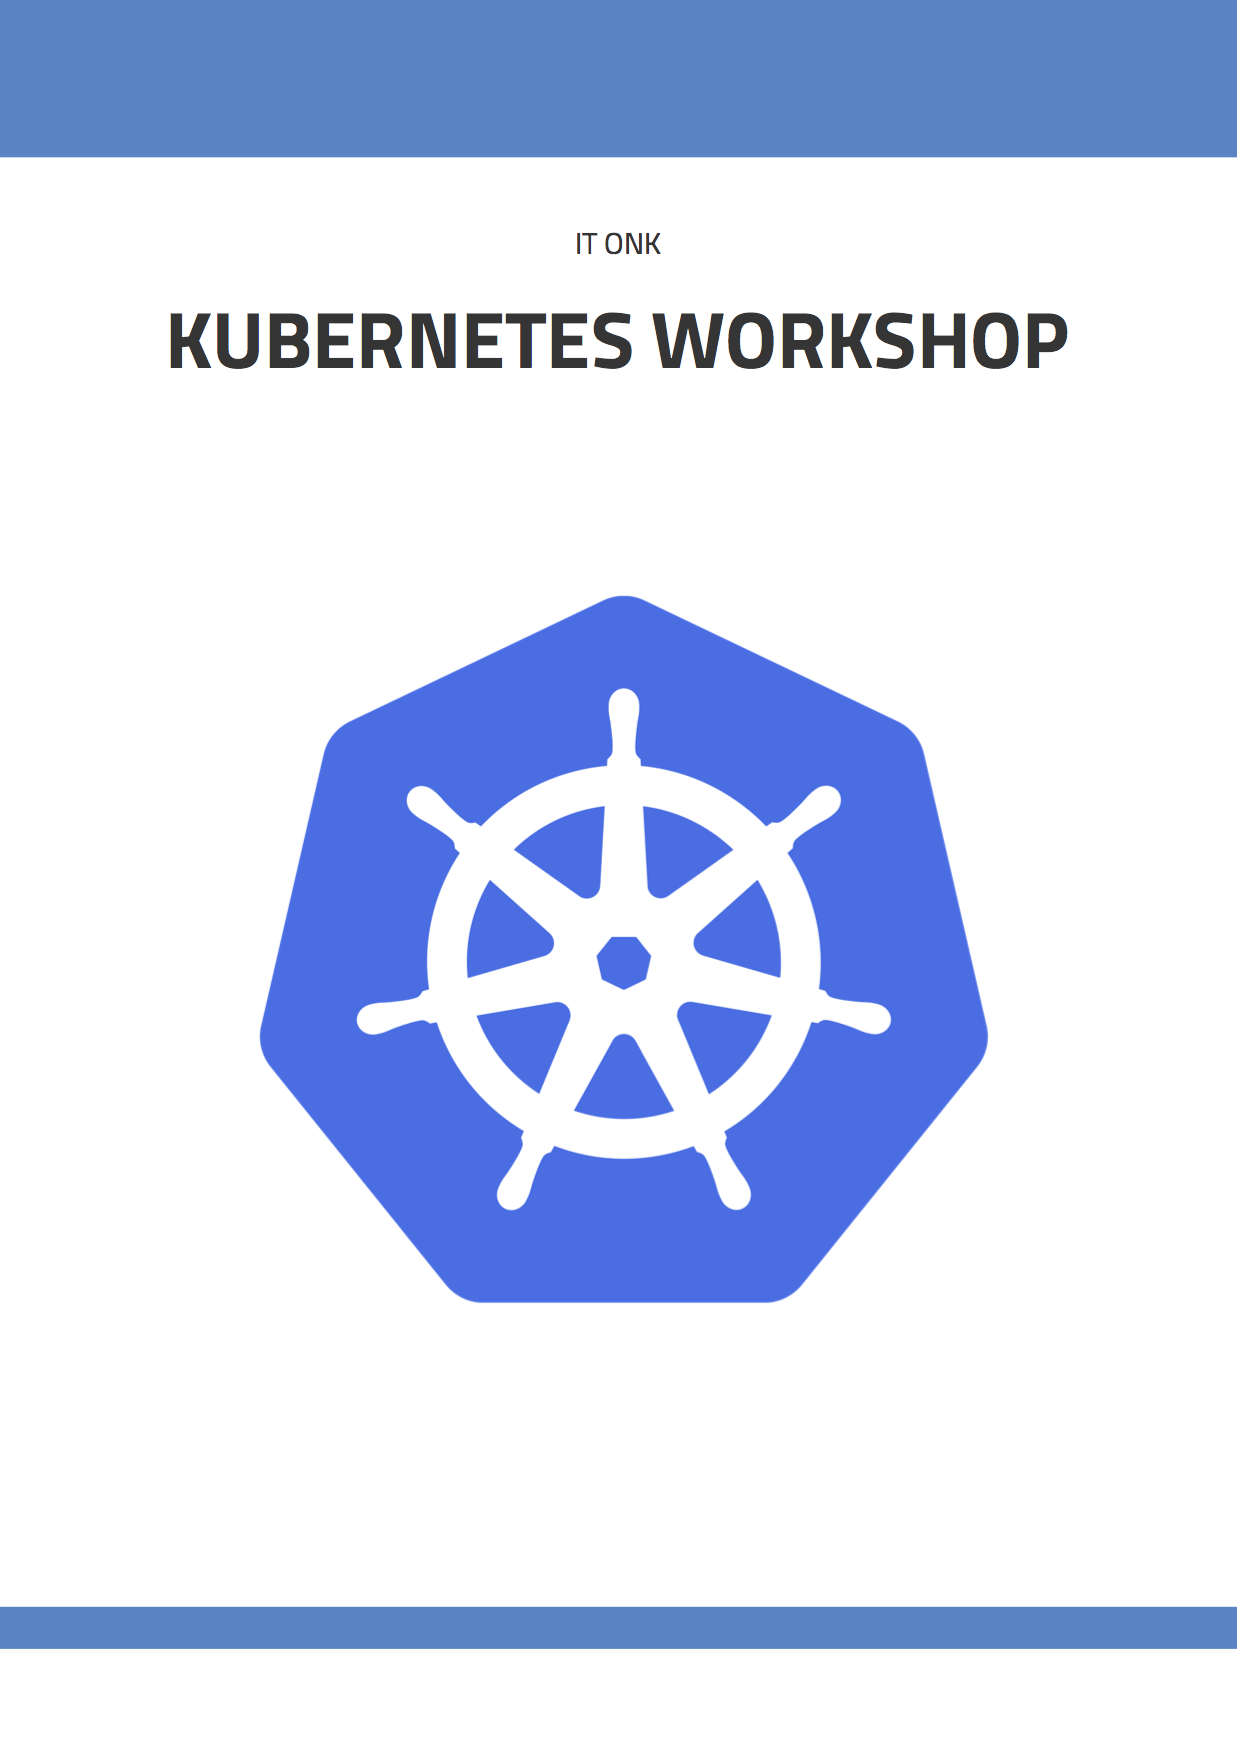
\includegraphics[align=t,width=5.5cm]{figures/workshop/module3_kubernetes}} & \textbf{Kubernetes workshop} \newline \textit{(13 sider)} \newline This workshop will provide the student with the ability to deploy containerized applications into the Raspberry Pi Kubernetes cluster. It will provide hands-on experience with using the command-line tool kubectl and familiarize the student with the presented concepts and how they can be leverage with Kubernetes. \\ 
\end{tabular}

\newpage

\noindent\begin{tabular}{p{6cm}p{7.5cm}}
\fbox{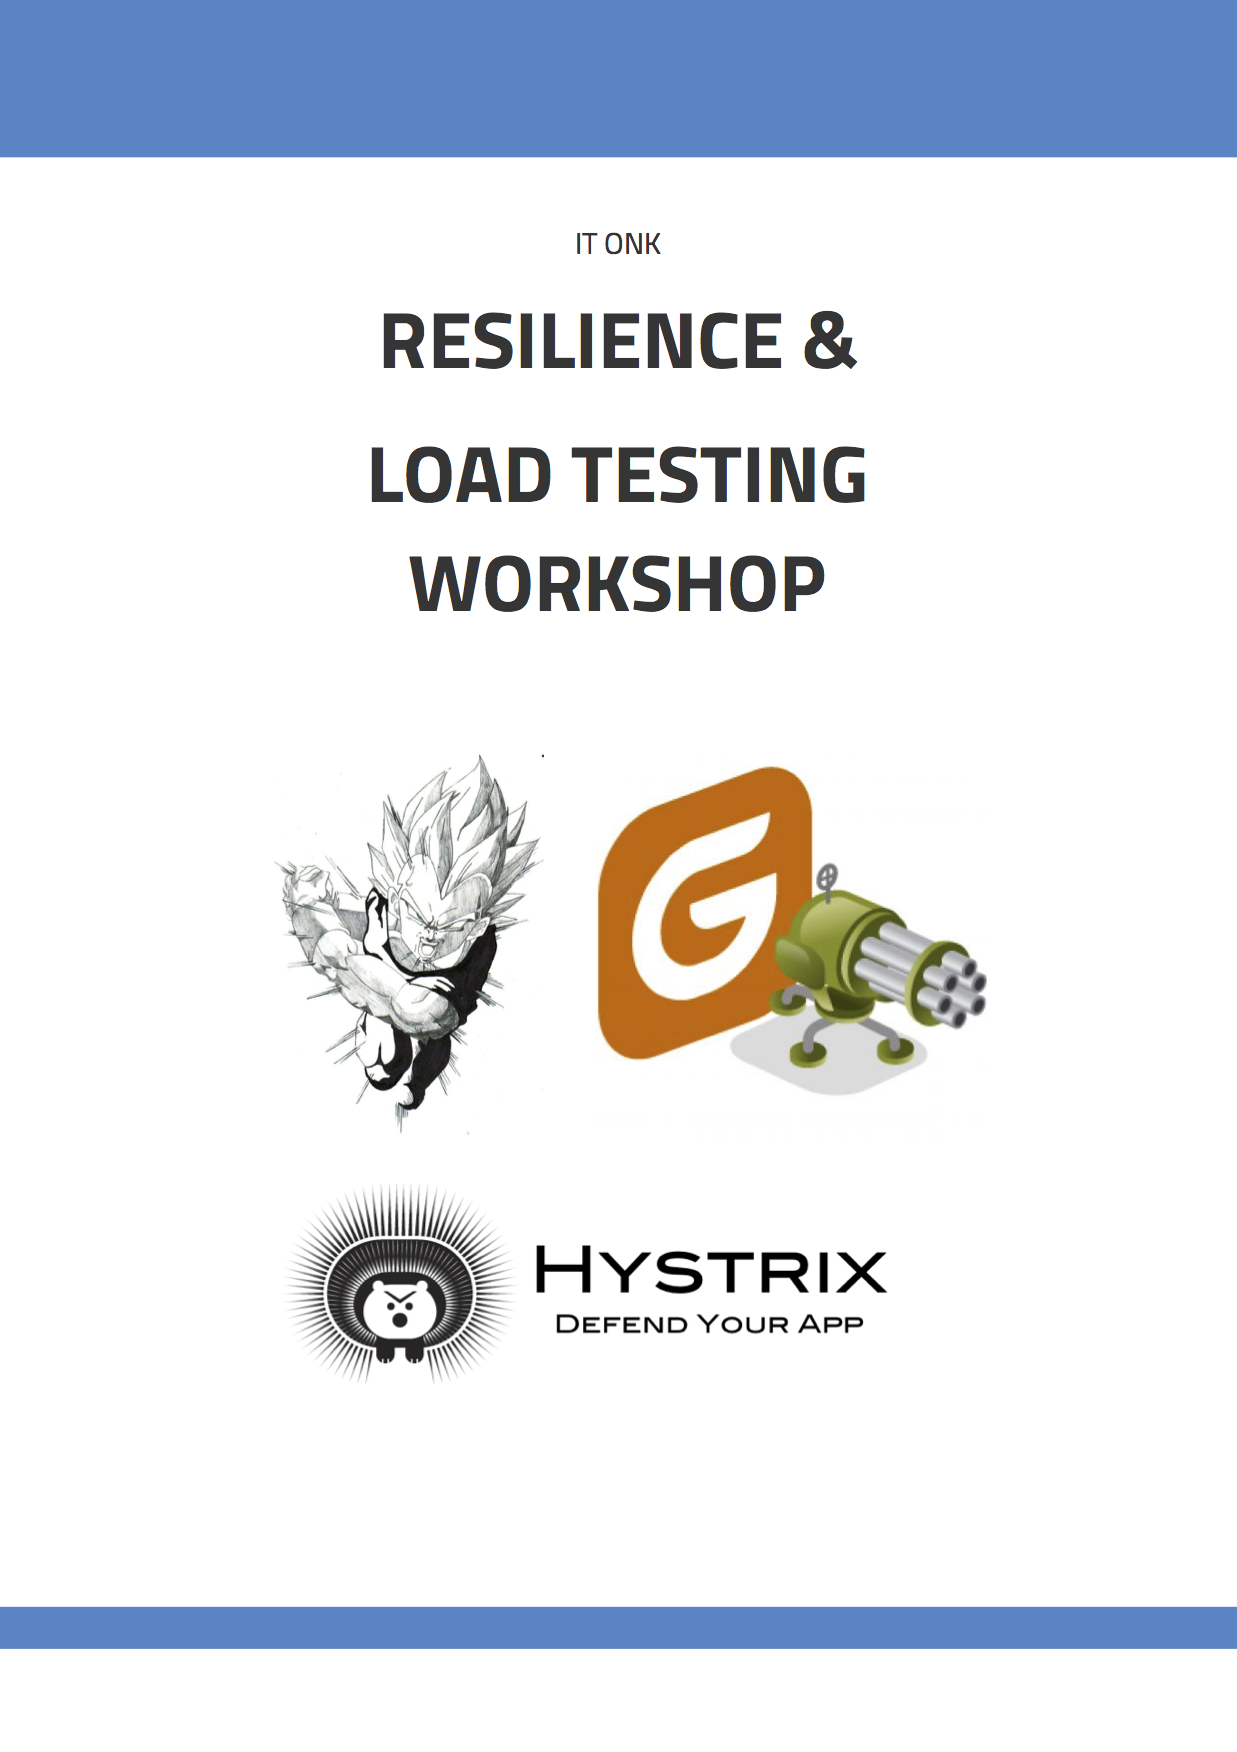
\includegraphics[align=t,width=5.5cm]{figures/workshop/module4_load_testing_resilience}} & \textbf{Resilience \& Load Testing workshop} \newline \textit{(19 sider)} \newline This workshop will provide the student with insight into the possible faults and errors that can happen in a distributed architecture. This workshop features already built docker images, the students has to configure and run different load-testing scenarios. The focus is on the effect of applying the Circuit Breaker pattern and using replication in Kubernetes.\\ 

\end{tabular}